% Poster for Menger Day 2019, Apr 1
% https://www.overleaf.com/6495666636xyhrjfrqtzzc


%%%%%%%%%%%%%%%%%%%%%%%%%%%%%%%%%%%%%%%%%
% Jacobs Landscape Poster
% LaTeX Template
% Version 1.0 (29/03/13)
%
% Created by:
% Computational Physics and Biophysics Group, Jacobs University
% https://teamwork.jacobs-university.de:8443/confluence/display/CoPandBiG/LaTeX+Poster
% 
% Further modified by:
% Nathaniel Johnston (nathaniel@njohnston.ca)
%
% Modified further still by:
% Abraham Nunes (nunes <at> dal <dot> ca)
%
% License:
% CC BY-NC-SA 3.0 (http://creativecommons.org/licenses/by-nc-sa/3.0/)
%
%%%%%%%%%%%%%%%%%%%%%%%%%%%%%%%%%%%%%%%%%

%----------------------------------------------------------------------------------------
%	PACKAGES AND OTHER DOCUMENT CONFIGURATIONS
%----------------------------------------------------------------------------------------

\documentclass[final]{beamer}

\usepackage[scale=1.24]{beamerposter} % Use the beamerposter package for laying out the poster
%%%%%%%%%%%%%%%%%%%%%%%%%%%%%%%%%%%%%%%%%%%%%%%%%%%%%%%%%%%%%
% About PEARC 19:  https://www.pearc19.pearc.org/call-for-participation
% Max poster size: 3.5 ft (1.1 m) wide by 4 ft (1.2 m) 
%%%%%%%%%%%%%%%%%%%%%%%%%%%%%%%%%%%%%%%%%%%%%%%%%%%%%%%%%%%%%

\usetheme{confposter} % Use the confposter theme supplied with this template

\setbeamercolor{block title}{fg=black,bg=white} % Colors of the block titles
\setbeamercolor{block body}{fg=black,bg=white} % Colors of the body of blocks
\setbeamercolor{block alerted title}{fg=white,bg=black} % Colors of the highlighted block titles
\setbeamercolor{block alerted body}{fg=black,bg=white} % Colors of the body of highlighted blocks
% Many more colors are available for use in beamerthemeconfposter.sty

%-----------------------------------------------------------
% Define the column widths and overall poster size
% To set effective sepwid, onecolwid and twocolwid values, first choose how many columns you want and how much separation you want between columns
% In this template, the separation width chosen is 0.024 of the paper width and a 4-column layout
% onecolwid should therefore be (1-(# of columns+1)*sepwid)/# of columns e.g. (1-(4+1)*0.024)/4 = 0.22
% Set twocolwid to be (2*onecolwid)+sepwid = 0.464
% Set threecolwid to be (3*onecolwid)+2*sepwid = 0.708

\newlength{\sepwid}
\newlength{\onecolwid}
\newlength{\twocolwid}
\newlength{\threecolwid}
\setlength{\paperwidth}{42in} % A0 width: 46.8in
\setlength{\paperheight}{48in} % A0 height: 33.1in
\setlength{\sepwid}{0.021\paperwidth} % Separation width (white space) between columns
\setlength{\onecolwid}{0.3\paperwidth} % Width of one column
\setlength{\twocolwid}{0.635\paperwidth} % Width of two columns
%\setlength{\threecolwid}{0.9\paperwidth} % Width of three columns
\setlength{\topmargin}{-0.5in} % Reduce the top margin size
%-----------------------------------------------------------
\usepackage{fancyhdr}
%\pagestyle{fancy}

%\setlength\headheight{1.38in} 

%\rhead{\includegraphics[width=\textwidth]{logoGAIL.jpg}}
\usepackage{graphicx}  % Required for including images

\usepackage{booktabs} % Top and bottom rules for tables
\usepackage{verbatim}
\usepackage{tikz}
\usepackage{siunitx}

%----------------------------------------------------------------------------------------
%	TITLE SECTION 
%----------------------------------------------------------------------------------------

\title{{\huge A Brief Introduction to GAIL (Guaranteed \\Automatic Integration Library) Version 2.3} }% Poster title

\author{Sou-Cheng T.~Choi, Jagadeeswaran Rathinavel, Xin Tong, Kan Zhang, Fred J.~Hickernell} % Author(s)

\institute{\texttt{hickernell@iit.edu}, Department of Applied Mathematics, Illinois Institute of Technology, Chicago %\\ [0.5ex]
		   %$^{2}$Department of Mathematics, Statistics, and Computer Science, University of Illinois, Chicago
		   } % Institution(s)

\begin{document}
	
\addtobeamertemplate{headline}{} 
{
	\begin{tikzpicture}[remember picture,overlay] 
	\node [anchor=north west, inner sep=2cm] at (current page.north west) {\includegraphics[height=11.5cm]{logoGAIL2.png}}; 
	\end{tikzpicture} 
}

\addtobeamertemplate{headline}{} 
{
	\begin{tikzpicture}[remember picture,overlay] 
	\node [anchor=north east, inner sep=2cm] at (current page.north east) {\includegraphics[height=11cm]{iit_high_res.png}}; 
	\end{tikzpicture} 
}

%----------------------------------------------------------------------------------------

\addtobeamertemplate{block end}{}{\vspace*{1.ex}} % White space under blocks
\addtobeamertemplate{block alerted end}{}{\vspace*{1.ex}} % White space under highlighted (alert) blocks

\setlength{\belowcaptionskip}{1.ex} % White space under figures
\setlength{\belowdisplayshortskip}{1.ex} % White space under equations

\begin{frame}[t] % The whole poster is enclosed in one beamer frame

\begin{columns}[t] % The whole poster consists of three major columns, the second of which is split into two columns twice - the [t] option aligns each column's content to the top

\begin{column}{\sepwid}\end{column} % Empty spacer column

\begin{column}{\onecolwid} % The first column

%----------------------------------------------------------------------------------------
%	OBJECTIVES
%----------------------------------------------------------------------------------------

\setbeamercolor{block alerted title}{fg=white,bg=IITgray} % Change the alert block title colors
\setbeamercolor{block alerted body}{fg=black,bg=white} % Change the alert block body colors

\begin{alertblock}{Overview}

GAIL algorithms compute answers of guaranteed accuracy for multidimensional integration as well as univariate integration,  function approximation and optimization:
%
\begin{itemize}
\item Requires only input function and error tolerance 
\item Theoretically sound stopping criterion
\item Well tested, documented, free, and open-source %algorithms that can be continually improved by new researchers.
%\item For high dimensional integration, uni-variate integration, function approximation and optimization 
\end{itemize}

\end{alertblock}

%----------------------------------------------------------------------------------------
%	INTRODUCTION
%----------------------------------------------------------------------------------------

\begin{block}{Introduction}
\begin{itemize}
\item Designing algorithms for a \emph{cone} of input functions allows us to prove that our stopping criteria are valid and information cost is optimal.

\item What is not observed about the function is not much worse than what is observed.
    % \item Automatic and adaptive approximation, optimization, or integration of functions in a cone with guarantee of accuracy is a relatively new paradigm.
    % \item Many adaptive numerical algorithms attempt to provide approximate solution that differ from the true solution no more than the user-specified error tolerance, but the stopping criterion are usually heuristic and not guaranteed to work in various scenarios.
    \item  We follow the philosophy  of  reproducible  research \& sustainable practices of  software development.
    % \item GAIL is an attempt to consolidate various guaranteed numerical algorithms born out of research and provide easily accessible software to the practitioners.
\end{itemize}
\end{block}

%----------------------------------------------------------------------------------------
%	METHODS
%----------------------------------------------------------------------------------------


\begin{block}{Approximation \& Optimization}

\begin{enumerate}\setlength\itemsep{1em}
\item \texttt{funappx\_g}: One-dimensional function approximation on bounded interval \cite{FunappxFunmin}
\item \texttt{funmin\_g}: Global minimum value of univariate function on a closed interval \cite{FunappxFunmin}
\end{enumerate}
\end{block}


\begin{block}{Option Pricing}

\begin{enumerate}\setlength\itemsep{1em}
\item \texttt{assetPath}: A class of discretized stochastic processes that model the values of an asset with respect to time \cite{ChoEtal18b}
\item \texttt{optPayoff}: A class of option payoffs based on asset paths \cite{ChoEtal18b}
\item \texttt{optPrice}: A class that computes the price of an option via (quasi-)Monte Carlo methods \cite{ChoEtal18b}
\end{enumerate}

\end{block}

\begin{block}{Integration}

\begin{enumerate} \setlength\itemsep{1em}

\item \texttt{integral\_g}: One-dimensional integration on bounded interval \cite{ChoEtal18b}
\item \texttt{meanMC\_g}: Monte Carlo (MC) method for estimating mean of a random variable \cite{meanMCcubMC}
\item \texttt{cubMC\_g}: MC method for  multiple integration \cite{meanMCcubMC}
\item \texttt{cubSobol\_g}: Quasi-Monte Carlo (QMC) method using Sobol' cubature for multiple integration \cite{cubSobol}
\item \texttt{cubLattice\_g}: QMC method using rank-1 lattices cubature for multiple integration \cite{cubLattice}
\item \texttt{cubBayesLattice\_g}: Bayesian cubature method using lattice sampling for multiple integration \cite{cubBayesLattice}
\item \texttt{meanMC\_CLT}: MC method with Central Limit Theorem (CLT) confidence intervals for estimating mean of a random variable \cite{ChoEtal18b}
\end{enumerate}

\end{block}



%----------------------------------------------------------------------------------------

\end{column} % End of the first column

\begin{column}{\sepwid}\end{column} % Empty spacer column

\begin{column}{\twocolwid} % Begin a column which is two columns wide (column 2)

\begin{columns}[t,totalwidth=\twocolwid] % Split up the two columns wide column

\begin{column}{\onecolwid}\vspace{-.8in} % The first column within column 2 (column 2.1)



%----------------------------------------------------------------------------------------
%	RESULTS
%----------------------------------------------------------------------------------------
\begin{block}{Example 1}
	\begin{figure}
		\centering
		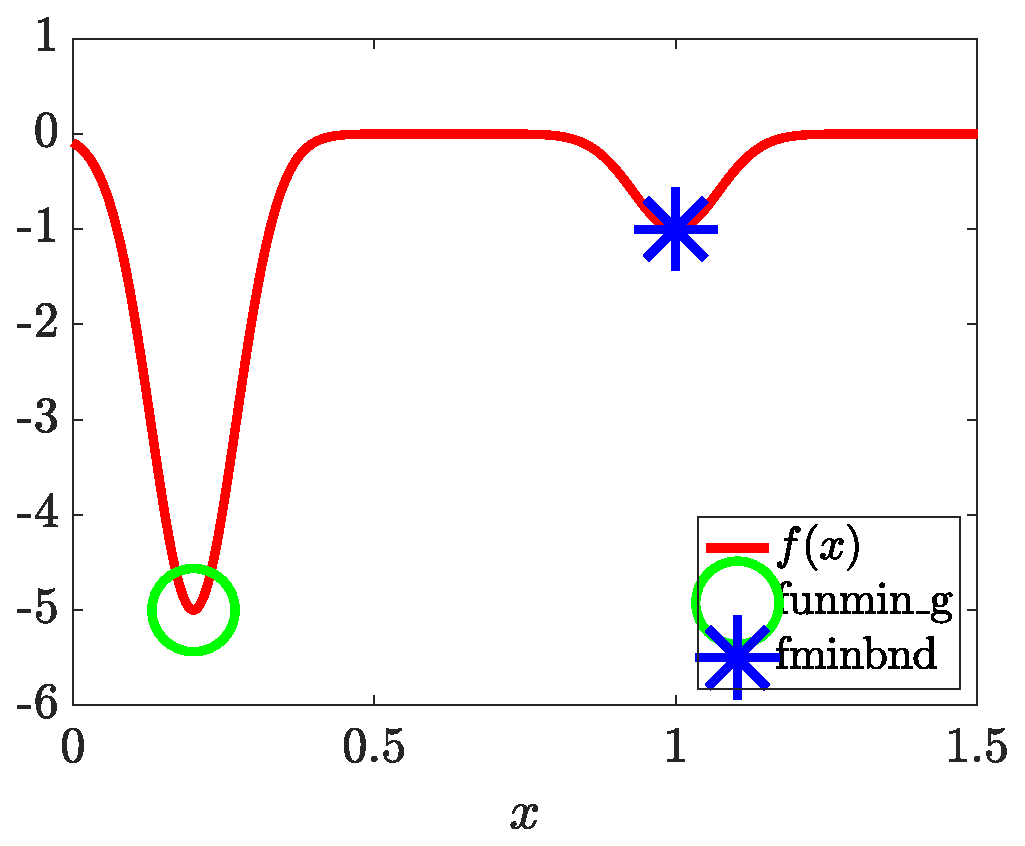
\includegraphics[width=0.76\linewidth]{abstract/humps.eps}
		\caption{We want to find the global minimum of 
		$f(x) = -5 e^{-100(x-0.2)^2}-e^{ -100(x-1)^2}$ for $x \in [0, 1.5]$.
		Our \texttt{funmin\_g} locates it but Matlab's \texttt{fminbnd} returns a local minimum.
	         Our algorithm automatically samples the function more often in spiky areas.}
		%\label{fig:min}
     \end{figure}
	
\end{block}	

%\begin{block}{\vspace{-11mm}Example 2}
%
%\begin{figure}
%	\centering
%	\includegraphics[width=1\linewidth]{cubSobol.png}
%	\caption[cubSobol]{Pricing geometric mean Asian call option by \texttt{cubSobol\_g} with $S_0=K=100$, $T=1$, $r=3\%$. $d$ is chosen uniformly from $1, 2, 4, 8, 16, 32, 64$; volatility is chosen uniformly from $10\%$ to $70\%$. The tolerance is \$0.01. The success rate is 100\% for this example.}
%	\label{fig:cubSobol}
%\end{figure}
%
%\end{block}
%
\begin{block}{\vspace{-11mm}Example 2}

\begin{figure}
	\centering
	\includegraphics[width=1.\linewidth]{"optPrice_guaranteed_time_full_Baker_d12_r1_2018-Sep-6b"}
	\caption[OptPrice guaranteed : FB]{Pricing  arithmetic mean Asian call option by \texttt{cubBayesLattice\_g}  with equal initial stock price and strike price $S_0 = K = 100$, maturity $T = 1/4$, risk-free interest rate $r =  5\%$, integral dimension $d = 13$, and volatility $\sigma = 0.5$. 
	The tolerances are $\epsilon=10^{-1}, 10^{-2}, 10^{-3}, 10^{-4}$. A sufficiently large sample size is chosen automatically to satisfy each $\epsilon$. The success rate is 100\% for this example.}
	\label{fig:optprice-guaranteed-FB}
\end{figure}

\end{block}

\begin{block}{Example 3}
\begin{table} % MATLAB Driver: KeisterCubatureExamplePEARC.m
       \centering
	\caption{Average performance of (quasi-)Monte Carlo algorithms in GAIL with automatic stopping 
	criteria for estimating the Keister integrals~\cite{keister1996multidimensional} of dimension $d$
	for $1000$ independent runs. \vspace{-3ex}}
	$
	%\arraycolsep=1.4pt\def\arraystretch{0.9}
        \begin{array}{l@{\qquad}r@{\quad}r@{\quad}r@{\quad}r@{\quad}r}	

	\input{abstract/KeisterPearcOut.txt} 
	\end{array}
	$
\end{table}
 \end{block}	

%----------------------------------------------------------------------------------------


\end{column} % End of column 2.1

%----------------------------------------------------------------------------------------


\begin{column}{\onecolwid}\vspace{-.8in} % The second column within column 2 (column 2.2)




%----------------------------------------------------------------------------------------



%----------------------------------------------------------------------------------------
%	FUTURE WORK
%----------------------------------------------------------------------------------------

\setbeamercolor{block alerted title}{fg=black,bg=dalblue} % Change the alert block title colors
\setbeamercolor{block alerted body}{fg=black,bg=white} % Change the alert block body colors

\begin{alertblock}{Ongoing Work}

\begin{itemize} 
%\item Release GAIL version 2.3 on Easter 2019
\item Submit GAIL to the Journal of Open Source Software
\item Make GAIL part of the multi-research group Quasi-Monte Carlo Community Software
\end{itemize}

\end{alertblock}

%----------------------------------------------------------------------------------------
%	REFERENCES
%----------------------------------------------------------------------------------------

\begin{block}{References}

\nocite{*} % Insert publications even if they are not cited in the poster
\small{\bibliographystyle{ieeetr}  %{abbrv}
\bibliography{abstract/gail_papers}\vspace{0.8in}}

\end{block}


%----------------------------------------------------------------------------------------
%	ACKNOWLEDGEMENTS
%----------------------------------------------------------------------------------------

\setbeamercolor{block title}{fg=black,bg=white} % Change the block title color

\begin{block}{Acknowledgements}

\small{\rmfamily{Our work is supported in part by grants NSF-DMS-1115392 and NSF-DMS-1522687. We thank all  GAIL contributors,
especially Yuhan Ding, Lan Jiang, Llu\'is Antoni Jim\'enez
Rugama, Aleksei Sorokin, and Yizhi Zhang.}} \\


\end{block}

%----------------------------------------------------------------------------------------
%	CONTACT INFORMATION
%----------------------------------------------------------------------------------------

\setbeamercolor{block alerted title}{fg=black,bg=dalblue} % Change the alert block title colors
\setbeamercolor{block alerted body}{fg=black,bg=white} % Change the alert block body colors



\end{column} % End of column 2.2

\end{columns} % End of the split of column 2 - any content after this will now take up 2 columns width

%----------------------------------------------------------------------------------------
%	IMPORTANT RESULT
%----------------------------------------------------------------------------------------

%\setbeamercolor{block alerted title}{fg=black,bg=dalgold} % Change the alert block title colors
%\setbeamercolor{block alerted body}{fg=black,bg=white} % Change the alert block body colors

%\begin{alertblock}{Highlights}

%Free open source software for multi-dimensional integration, one-dimensional functional approximation and optimization with guaranteed user specified error tolerance.

%\end{alertblock} 

%----------------------------------------------------------------------------------------
\begin{column}{\sepwid}\end{column}

\begin{column}{\twocolwid} % Begin a column which is two columns wide (column 2)

\begin{columns}[t,totalwidth=\twocolwid] % Split up the two columns wide column again

\begin{column}{\onecolwid} % The first column within column 2 (column 2.1)

%----------------------------------------------------------------------------------------
%	MATHEMATICAL SECTION
%----------------------------------------------------------------------------------------


%----------------------------------------------------------------------------------------

\end{column} % End of column 2.1
\begin{column}{\sepwid}\end{column}
\begin{column}{\onecolwid} % The second column within column 2 (column 2.2)



%----------------------------------------------------------------------------------------

\end{column} % End of column 2.2

\begin{column}{\onecolwid} % The third column within column 2 (column 2.3)
	

%----------------------------------------------------------------------------------------
	
\end{column} % End of column 2.3

\end{columns} % End of the split of column 2

\end{column}

\end{column} % End of the second column

\begin{column}{\sepwid}\end{column} % Empty spacer column

\begin{column}{\onecolwid} % The third column


%----------------------------------------------------------------------------------------

\end{column} % End of the third column

\end{columns} % End of all the columns in the poster

\end{frame} % End of the enclosing frame

\end{document}
